% %NOTE:
% % CHECKED WITH SLIDES: YES!
% % CHECKED WITH EXERCISES: NO -- TODO
% % MISSING: -

\section{RTOS: Real-Time OS}

\begin{definition}[Real-time Operating System]
A real-time operating system is an operating system that 
supports the construction of real-time systems.
\end{definition}

\subsection{Desktop OS not suited}
\begin{itemize}[noitemsep]
\item Monolithic kernel too feature rich. Not modular, configurable, modifiable
\item Too much space
\item Not power optimized
\item Timing uncertainty too large
\end{itemize}

\subsection{Properties of RTOS/Embedded OS}
\begin{itemize}[noitemsep]
\item Configurability: no single RTOS will fit all needs. Reduce overhead. Examples: Remove unused functions at compile time
\item Device drivers handled by tasks. Meaning everything goes through the scheduler (device drivers rely on the kernel)
\item Interrupts employed by any process. Time to handle interrupts need to be considered
\item Protection mechanism not always necessary. ES designed for a single purpose, rarely untested programs - SW considered reliable. Task do their own IO instructions instead of kernel call.
\end{itemize}

\subsection{Requirements}
\subsubsection{Timing Behavior}
The timing behavior of the OS must be predictable. For all services of the OS, there has to be an upper bound on the execution time. RTOS must be deterministic.

\subsubsection{Timing}
OS must manage the timing and scheduling. Must be aware of deadlines and provide precise time services with high resolution.

\subsubsection{Fast}
The OS must be fast. In general, practically important.

\subsection{Functionality of RTOS-Kernels}
\begin{itemize}[noitemsep]
\item Execution of quasi-parallel tasks on a processor using processes or threads (lightweight process). Providing and maintaining process states, process queuing, preemptive tasks, fast context switching, quick interrupt handling
\item CPU scheduling (guaranteeing deadlines, minimizing process waiting times, fairness in granting resources such as computing power)
\item Process synchronization (critical sections, semaphores, monitors, mutual exclusion)
\item Inter-process communication (buffering)
\item Support of a real-time clock as an internal time reference
\end{itemize}

\subsection{Context-Switch}
\begin{figure}[ht]
	\centering
  	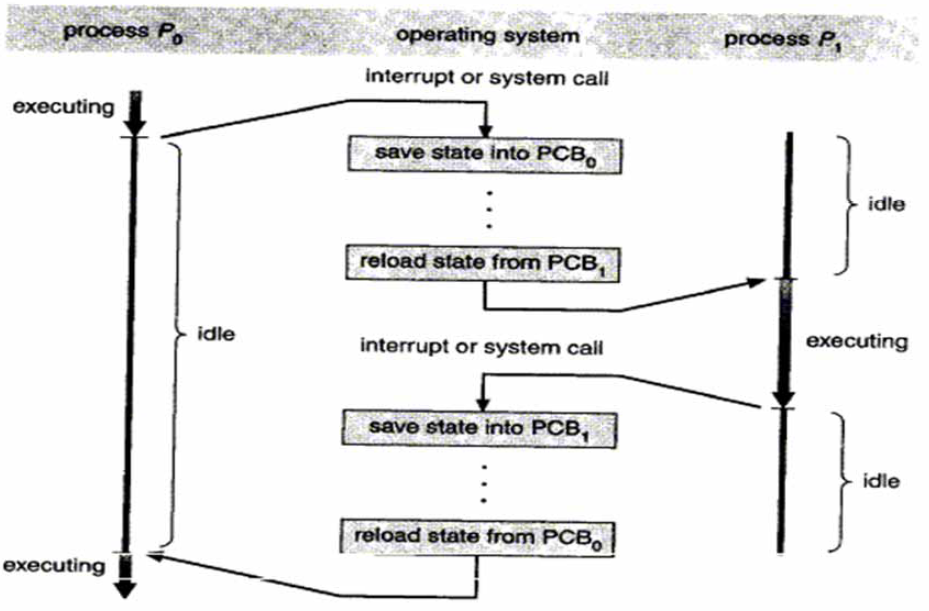
\includegraphics[scale=0.3]{img/6_context_switch.png}
	\caption{Context switch from process 0 to process 1 and back}
	\label{fig:context_switch}
\end{figure}


\subsection{Process states}
\begin{itemize}[noitemsep]
\item Run: A task enters this state as it starts executing on the processor
\item Ready: State of those tasks that are ready to execute but cannot be executed because the processor is assigned to another task
\item Wait: A task enters this state when it executes a synchronization primitive to wait for an event, e.g. a wait primitive on a semaphore. In this case, the task is inserted in a queue associated with the semaphore. The task at the head is resumed when the semaphore is unlocked by a signal primitive.
\item Idle: A periodic job enters this state when it completes its execution and has to wait for the beginning of the next period
\end{itemize}

\begin{figure}[ht]
	\centering
  	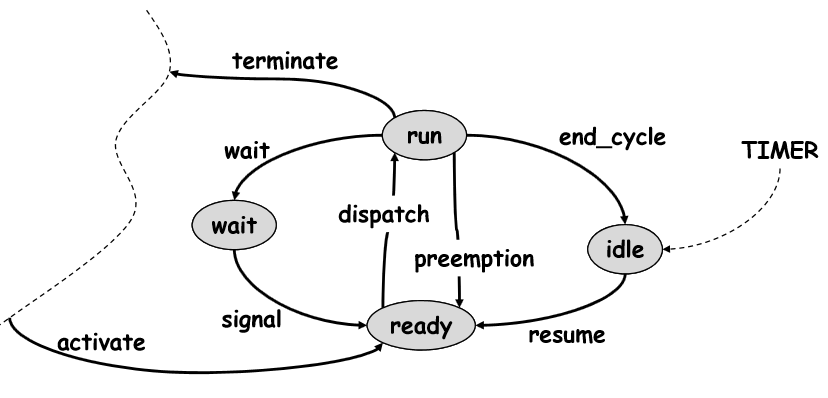
\includegraphics[scale=0.5]{img/6_process_states.png}
	\caption{State diagram of process states.}
	\label{fig_process_states}
\end{figure}

\subsection{Threads}
\begin{definition}[Thread]
A 
thread
is an execution stream within the context of a thread state; e.g., a thread is a basic unit of CPU utilization
\end{definition}

\begin{itemize}[noitemsep]
\item key difference between processes and threads: multiple threads share parts of their state (shared memory, own register and stack)
\item Faster to switch between threads (user-level threads)
\item an application will have a separate  thread for each distinct activity
\item Thread Control Block (TCB) stores information needed to manage and schedule a thread
\end{itemize}

\subsubsection{Process Management}
\begin{itemize}[noitemsep]
\item Typical os: synchronization and mutual exclusion is performed via semaphores and monitors
\item In real-time OS, special semaphores and a deep integration into scheduling is necessary (priority inheritance protocols)
\item Initializations of internal data structures (tables, queues, task description blocks, semaphores)
\end{itemize}


\subsection{Synchronous Communication}
\begin{itemize}[noitemsep]
\item rendez-vous
\item Have to wait for each other
\item Problem in dynamic RTS: Estimating the maximum blocking time for a process rendez-vous
\item In static RTS: the problem can be solved off-line by transforming all synchronous interactions into precedence constraints
\end{itemize}

\subsection{Asynchronous Communication}
\begin{itemize}[noitemsep]
\item More suited for real-time systems
\item Tasks do not have to wait for each other.
\item sender just deposits its message into a channel and continues its execution
\item receiver can directly access the message if at least a message has been deposited into the channel
\item Shared memory buffer, FIFO-queue. Often has fixed capacity
\item Problem: Blocking behavior if channel is full or empty. Solved by cyclic (overriding) buffers
\end{itemize}

\subsection{Class of Kernels}
\subsubsection{Class 1 - Fast Proprietary Kernels}
For hard real-time systems, these kernels are questionable, because they are designed to be fast, rather than to be predictable in every respect.
Examples: VxWORKS

\subsubsection{Class 2 - Extensions to Standard OSs}
Real-time extensions to standard OS: Attempt to exploit comfortable main stream OS. RT-kernel running all RT-tasks. Standard-OS executed as one task.
Pro: Crash of standard-OS does not affect RT-tasks. Con: RT-tasks cannot use Standard-OS services; less comfortable than expected 

\subsubsection{Class 3 - Research Systems}
\begin{itemize}[noitemsep]
\item trying to avoid limitations of overhead memory protection
\item temporal protection of computing resources 
\item quality of service (QoS) control
\item formally verified kernel properties
\end{itemize}

\cleardoublepage